\documentclass[journal]{IEEEtran}
	\usepackage{graphicx}
	\usepackage{caption}
	\usepackage{hyperref}
    \usepackage{float}
    
\begin{document}

\title{Group 67 - Research Paper}
\author{Deep Learning for Object Recognition on a Mobile Robot\\
Julian Weisbord, Miles McCall, Michael Rodriguez \\
Oregon State University \\
CS 463 Spring 2018 \\
}
\maketitle

\begin{abstract}
The research paper is the write up of our research findings. It includes the methods and technologies we tested in our project and the results from those experiments. This document acts as the conclusion to the research aspect of our project.
\end{abstract}

\begin{IEEEkeywords}
	Deep Learning, Online Learning, Object Recognition, Mobile Robot
\end{IEEEkeywords}

\tableofcontents
\listoffigures

\section{Introduction}
Our project is research oriented, meaning we spent time experimenting and investigating different technologies and techniques. Our software pipeline has several major programs that interact with each other to collect and process of our data. For each of these steps we looked into alternative solutions to the problem, and analyzed details such cost benefit analyses and the potential to scale technologies as the classification model grows. 
   
\section{Areas of Research}
While the main goal of our project was to create a fully functional software pipeline, we incorporated research into every component of the pipeline. The problem of sequential online learning is not solved by one perfect algorithm or software library
    
  \subsection{Data Gathering}

  \subsection{Image Cropping}
  
  \subsection{Neural Network Model}
  
  \subsection{Online Learning Techniques}
  
\section{Results} 
  \begin{figure}[H]
    \begin{center}
      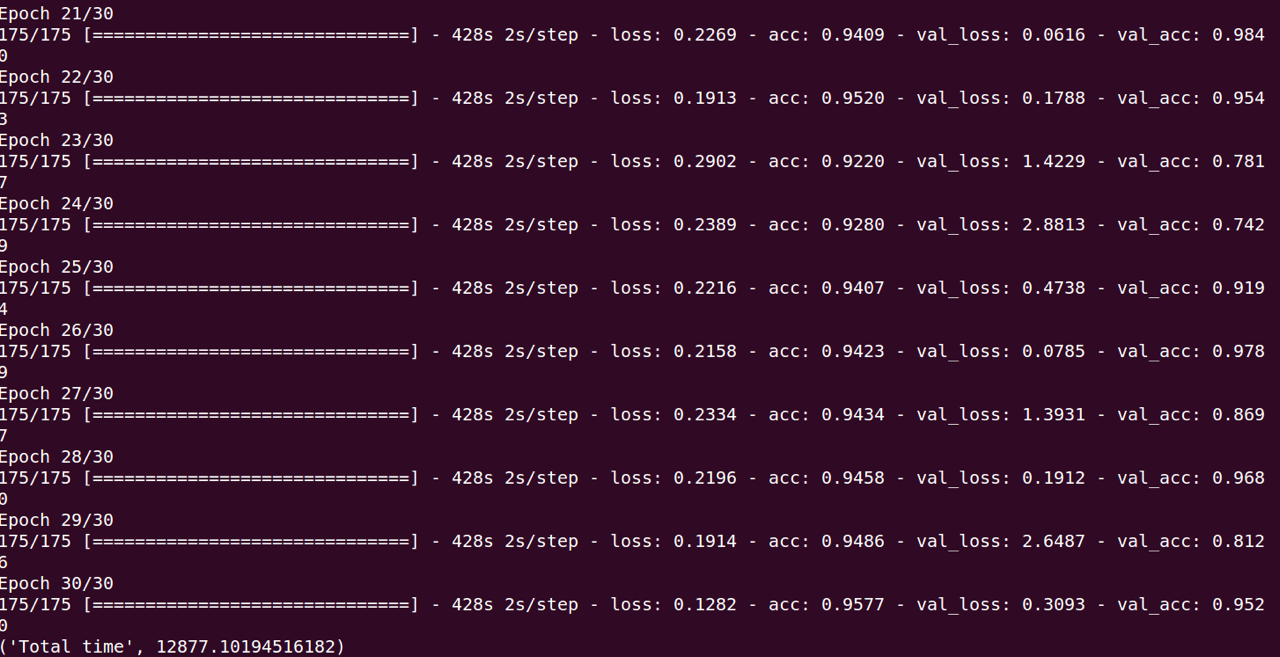
\includegraphics[width=\linewidth]{pictures/results.png}
          \caption{Accuracy Training}
    \end{center}
  \end{figure}

\begin{figure}[H]
  \begin{center}
    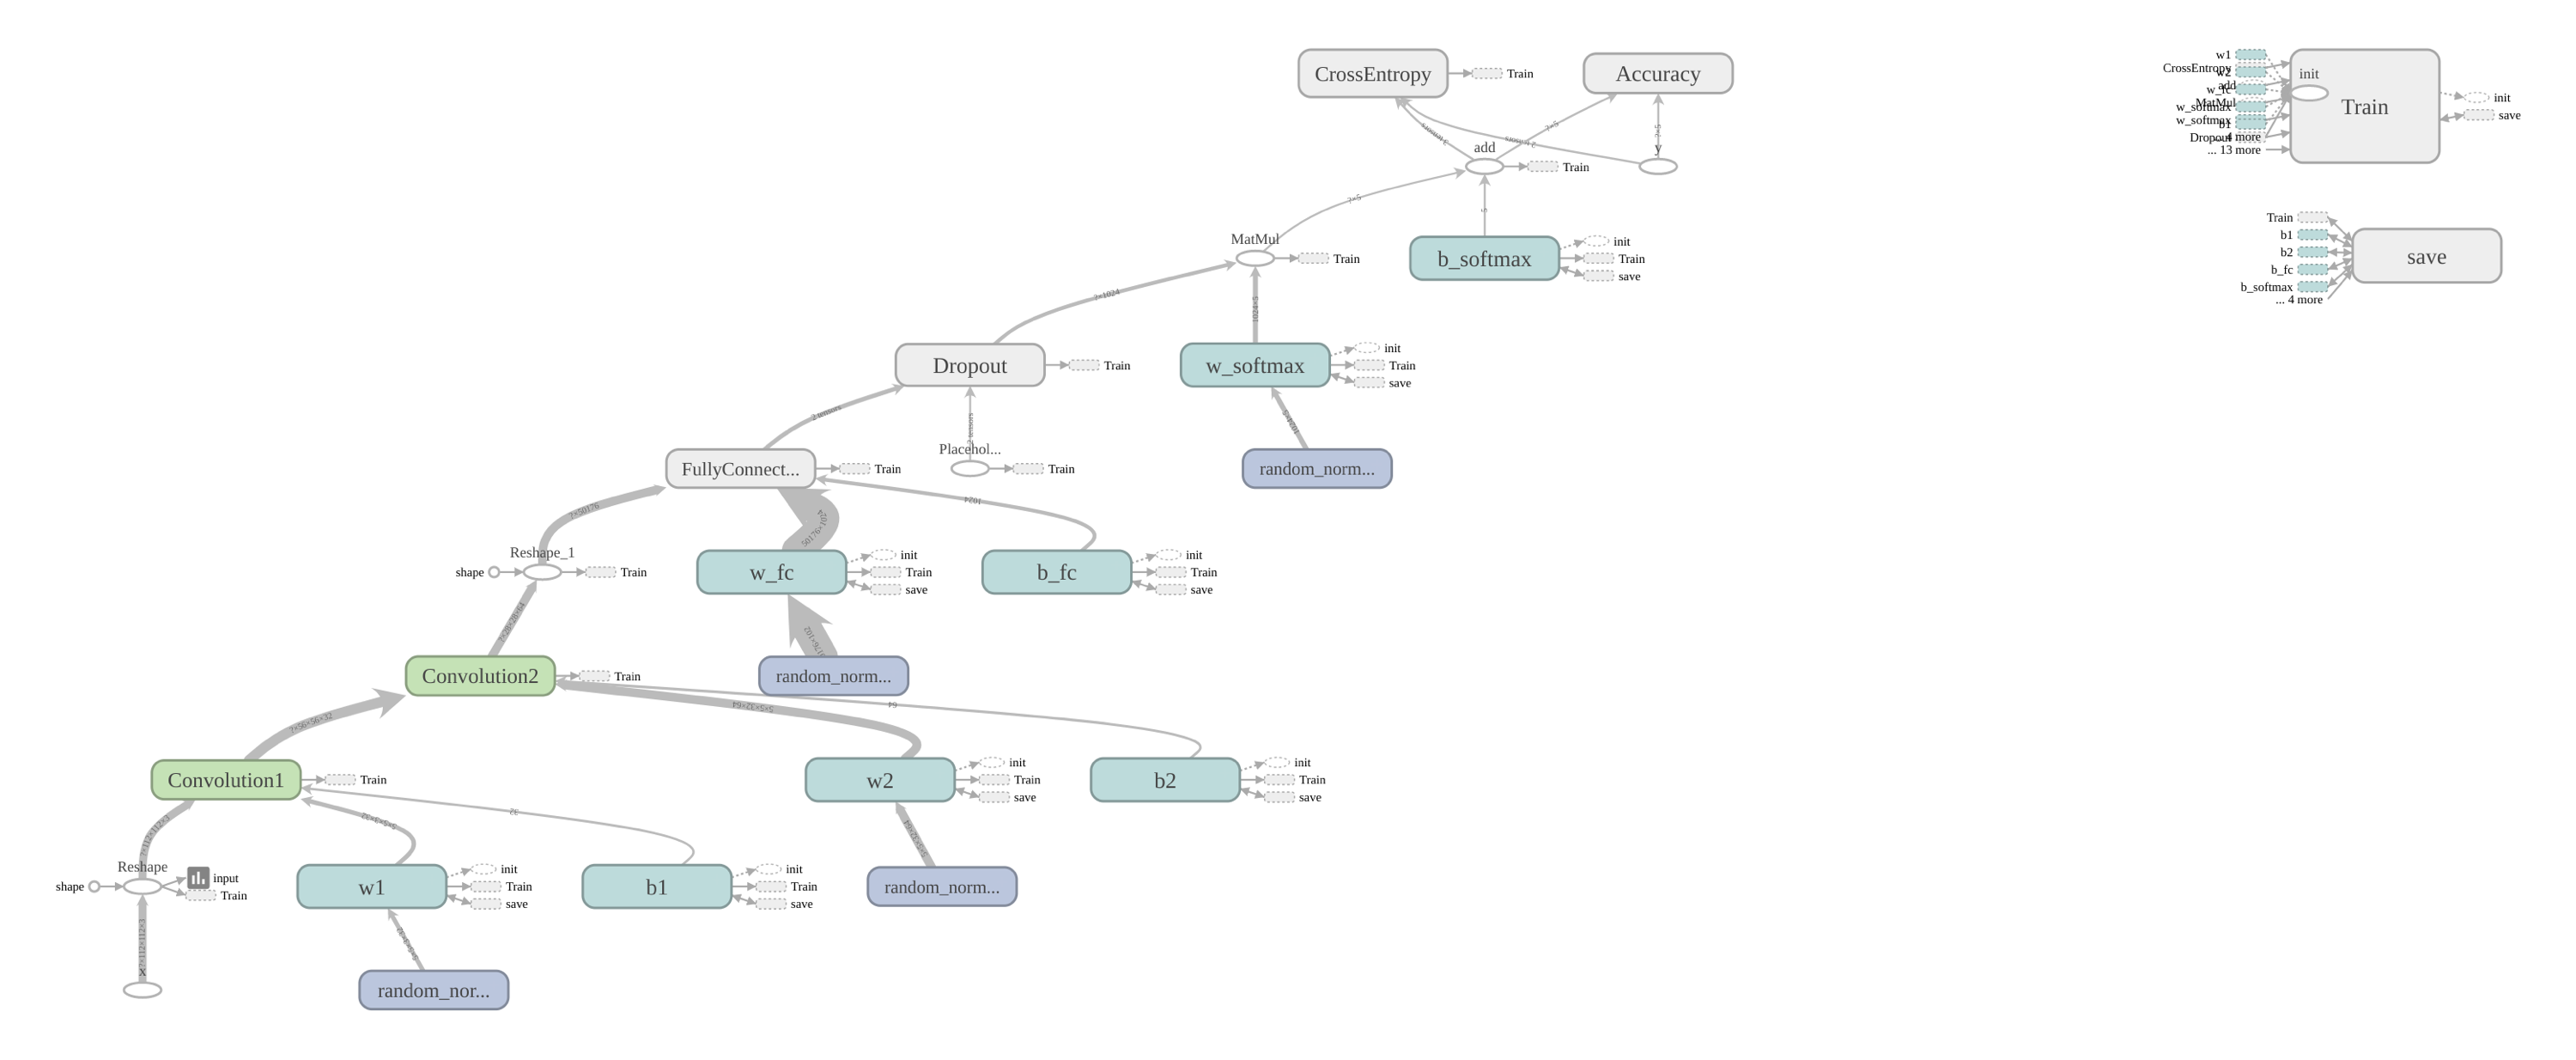
\includegraphics[width=\linewidth]{pictures/model.png}
        \caption{Network Model}
  \end{center}
\end{figure}

\section{Conclusion}

\appendix
\newpage
%\bibliography{research}
%\bibliographystyle{IEEEtran}
\end{document}


